\documentclass[a4paper,12pt]{article}
	
\usepackage[T2A]{fontenc}			
\usepackage[utf8]{inputenc}			
\usepackage[english,russian]{babel}	

\usepackage[
bookmarks=true, colorlinks=true, unicode=true,
urlcolor=black,linkcolor=black, anchorcolor=black,
citecolor=black, menucolor=black, filecolor=black,
]{hyperref}

\usepackage{color}
\usepackage{caption}


\usepackage{amsmath,amsfonts,amssymb,amsthm,mathtools} 
\usepackage{wasysym}

\usepackage{graphicx}
%\usepackage[cache=false]{minted}
\usepackage{cmap}
\usepackage{indentfirst}

\usepackage{listings} 
\usepackage{fancyvrb}
\usepackage{slashbox}

\usepackage{geometry}
\geometry{left=2cm}
\geometry{right=1.5cm}
\geometry{top=1cm}
\geometry{bottom=2cm}

\setlength{\parindent}{5ex}
\setlength{\parskip}{0.5em}

\usepackage{titlesec}
\usepackage{pgfplots}
\usepackage{filecontents}
\usetikzlibrary{datavisualization}
\usetikzlibrary{datavisualization.formats.functions}

\DeclareCaptionFont{white}{\color{white}}
\DeclareCaptionFormat{listing}{\colorbox{gray}{\parbox{\textwidth}{#1#2#3}}}
\captionsetup[lstlisting]{format=listing,labelfont=white,textfont=white}
\lstloadlanguages{% Check Dokumentation for further languages ...
C,
C++,
csh,
Java
}

\definecolor{red}{rgb}{0.6,0,0} % for strings
\definecolor{blue}{rgb}{0,0,0.6}
\definecolor{green}{rgb}{0,0.8,0}
\definecolor{cyan}{rgb}{0.0,0.6,0.6}

\lstset{ %
language=Lisp,                 % выбор языка для подсветки
basicstyle=\small\sffamily, % размер и начертание шрифта для подсветки кода
numbers=left,               % где поставить нумерацию строк (слева\справа)
numberstyle=\tiny,           % размер шрифта для номеров строк
stepnumber=1,                   % размер шага между двумя номерами строк
numbersep=5pt,                % как далеко отстоят номера строк от подсвечиваемого кода
showspaces=false,
backgroundcolor=\color{white},         
showstringspaces=false,      % показывать или нет пробелы в строках
showtabs=false,             % показывать или нет табуляцию в строках
frame=single,              % рисовать рамку вокруг кода
tabsize=2,                 % размер табуляции по умолчанию равен 2 пробелам
captionpos=t,              % позиция заголовка вверху [t] или внизу [b] 
breaklines=true,           % автоматически переносить строки (да\нет)
breakatwhitespace=false, % переносить строки только если есть пробел
escapeinside={\%*}{*)}
}

% Для измененных титулов глав:
\definecolor{gray75}{gray}{0.75} % определяем цвет
\newcommand{\hsp}{\hspace{20pt}} % длина линии в 20pt
% titleformat определяет стиль
\titleformat{\chapter}[hang]{\Huge\bfseries}{\thechapter\hsp\textcolor{gray75}{|}\hsp}{0pt}{\Huge\bfseries}

\begin{document}
	
\begin{figure}[h!]
	\begin{center}
		{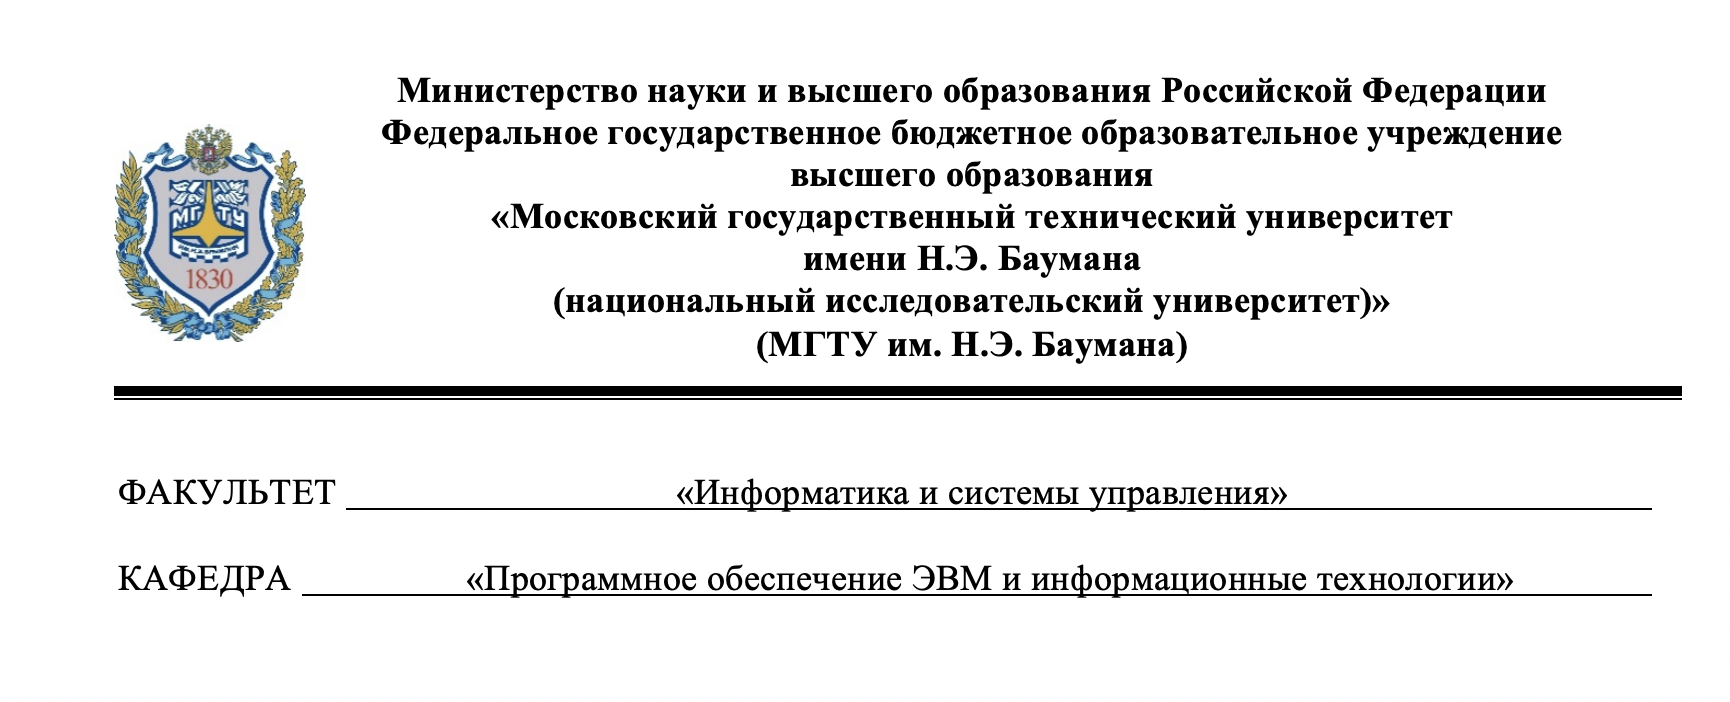
\includegraphics[width = \textwidth]{titul.png}}
	\end{center}
\end{figure}

\vspace*{20mm}

\huge
\begin{center}
	Лабораторная работа №2
\end{center}


\vspace*{50mm}

\large
\begin{flushleft}
	Студент: Луговой Д.М. \\
	Группа: ИУ7-61Б \\
	Преподаватель: Толпинская Н.Б.
\end{flushleft}

\vspace*{60mm}

\large
\begin{center}
	Москва, 2020 г.
\end{center}

\thispagestyle{empty}

\newpage
\vspace*{10mm}
\textbf{Цель работы}: приобрести навыки использования списков и стандартных функций Lisp.\\

\textbf{Задачи работы}: изучить способ использования списков для фиксации информации, внутреннее представление одноуровневых и структурированных списков, методы их обработки с использованием базовых функций Lisp.

\begin{enumerate}
\item \textbf{Базис LISP}

Базис языка – это необходимый минимальный набор конструкций, которые должные обязательно присутствовать, чтобы при их помощи составлять команды. Базис языка Lisp образуют атомы, структуры, базовые функции и функционалы. 

\item \textbf{Классификация функций}

Функция есть однозначное отображение множества исходных данных на множество её значений.
Функции классифицируются на:
\begin{itemize}
\item Чистые математические функции - принимают фиксированное количество аргументов
\item Формы – принимают не фиксированное количество аргументов или обрабатывают аргументы по разному
\item Функционалы (высших порядков) – используют другие функции в качестве аргументов или вырабатывают в качестве результатов.
\item Базисные функции
\begin{itemize}
\item Селекторы (функции доступа) - car, cdr
\item Конструкторы (функции создания структур) - cons, list
\item Предикаты - atom, null, listp, consp
\item Функции сравнения - eq, eql, equal, =, equalp
\end{itemize}
\end{itemize}

\item \textbf{Представление списков в памяти}

Список – это структура данных. Может быть пустой и непустой. В памяти представлен списочной ячейкой, содержащей указатели на голову списка и на его хвост. Голова списка представляет из себя S-выражение, хвост является списком. Список может быть пустым. В  Lisp возможны два типа представления пустого списка: пара пустых скобок и специальный символ Nil. 
\newpage
\item \textbf{Функции CAR и CDR}

CAR и CDR являются базовыми функциями доступа к данным. CAR принимает точечную пару или пустой список в качестве аргумента и возвращает первый элемент или nil, соответственно. CDR принимает точечную пару или пустой список и возвращает список состоящий из всех элементов, кроме первого. Если в списке меньше двух элементов, то возвращается Nil.
\end{enumerate}

\vspace*{10mm}

{\LARGE Задание №1}\\

Что будет в результате вычисления выражений?
\begin{enumerate}
\item (CAADR ‘((blue cube) (red pyramid)))\\
Результат: red
\begin{figure}[ht!]
\center{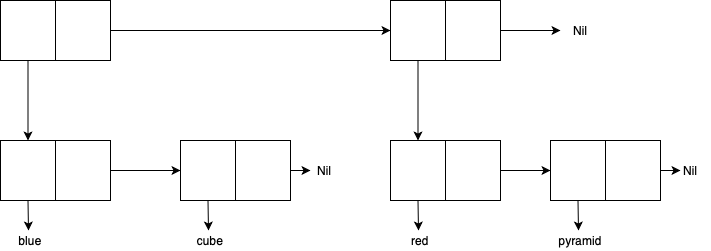
\includegraphics[scale=0.6]{FaLP1.png}}
\end{figure}
\item (CDAR ‘((abc) (def) (ghi)))\\
Результат: Nil
\begin{figure}[ht!]
\center{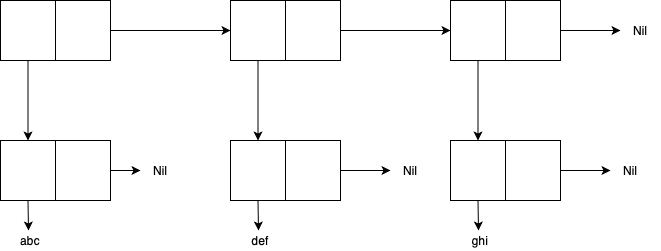
\includegraphics[scale=0.6]{FaLP2.png}}
\end{figure}
\item (CADR ‘((abc) (def) (ghi)))\\
Результат: (def)
\item (CADDR ‘((abc) (def) (ghi)))\\
Результат: (ghi)\\
\end{enumerate}

\newpage
\vspace*{10mm}

{\LARGE Задание №2}\\

Напишите результат вычисления выражений:
\begin{enumerate}
\item (list 'Fred 'and Wilma)\\
Результат: The variable WILMA is unbound. Wilma не может быть вычислено.
\item (list 'Fred '(and Wilma))\\
Результат: (Fred (and Wilma))
\item (cons Nil Nil)\\
Результат: (NIL)
\item (cons T Nil)\\
Результат: (T)
\item (cons Nil T)\\
Результат: (Nil . T)
\item (list Nil)\\
Результат: (Nil)
\item (cons (T) Nil)\\
Результат: The function COMMON-LISP: T is undefined. T не является функцией.
\item (list ‘(one two) ‘(free temp))\\
Результат: ((one two) (free temp))
\item ((cons 'Fred '(and Wilma))\\
Результат: (Fred and Wilma)
\item (cons ‘Fred ‘(Wilma))\\
Результат: (Fred Wilma)
\item (list Nil Nil)\\
Результат: (Nil Nil)
\item (list T Nil)\\
Результат: (T Nil)
\item (list Nil T)\\
Результат: (Nil T)
\item (cons T (list Nil))\\
Результат: (T Nil)
\item (list (T) Nil)\\
Результат: The function COMMON-LISP: T is undefined. T не является функцией.
\item (cons ‘(one two) ‘(free tmp))\\
Результат: ((one two) free tmp)\\
\end{enumerate}


{\LARGE Задание №3}\\

Написать функцию
\begin{enumerate}
\item (f ar1 ar2 ar3 ar4), возвращающую ((ar1 ar2) (ar3 ar4)):
\begin{itemize}
\item (defun f (ar1 ar2 ar3 ar4) (list (list ar1 ar2) (list ar3 ar4)))  
\item (defun f (ar1 ar2 ar3 ar4) `((,ar1 ,ar2) (,ar3 ,ar4)))
\item (defun f (ar1 ar2 ar3 ar4) (cons (cons 1 (cons 2 NIl))(cons (cons 3 (cons 4 Nil)) Nil)))
\end{itemize}
\begin{figure}[ht!]
\center{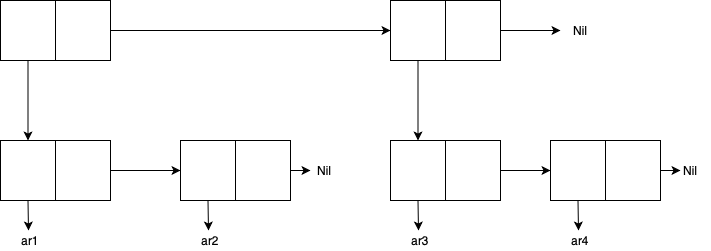
\includegraphics[scale=0.6]{FaLP3.png}}
\end{figure}

\item (f ar1 ar2), возвращающую ((ar1) (ar2)):\\
Функция: (defun f (ar1 ar2) (list (list ar1) (list ar2)))
\begin{figure}[ht!]
\center{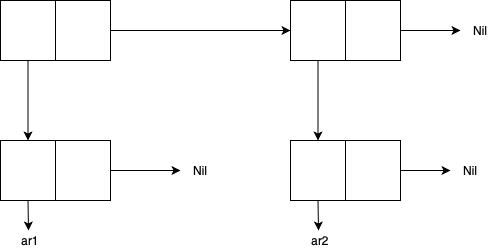
\includegraphics[scale=0.6]{FaLP4.png}}
\end{figure}

\item (f ar1), возвращающую (((ar1))):\\
Функция: (defun f (ar1) (list (list (list ar1))))
\begin{figure}[ht!]
\center{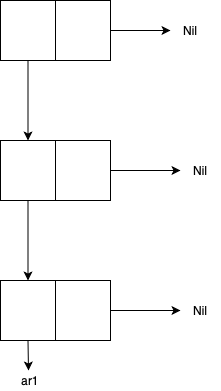
\includegraphics[scale=0.6]{FaLP5.png}}
\end{figure}
\end{enumerate}

\end{document}

